\documentclass[11pt,a4paper]{article}

\usepackage[a4paper,margin=2.3cm]{geometry}
\usepackage{fontspec}
\usepackage{graphicx}
\usepackage{xcolor}
\usepackage{tabularx}
\usepackage{longtable}
\usepackage{booktabs}
\usepackage{enumitem}
\usepackage{array}
\usepackage{hyperref}
\usepackage{fancyhdr}
\usepackage{titlesec}
\usepackage{caption}
\usepackage{float}

\setmainfont{Latin Modern Roman}
\setsansfont{Latin Modern Sans}
\setmonofont{Latin Modern Mono}

\renewcommand{\contentsname}{Índice}
\renewcommand{\figurename}{Figura}
\renewcommand{\tablename}{Tabla}

\definecolor{FieBlue}{HTML}{1E3A8A}
\definecolor{FieSlate}{HTML}{334155}
\definecolor{FieLight}{HTML}{F8FAFC}
\definecolor{FieLine}{HTML}{CBD5E1}

\hypersetup{
  colorlinks=true,
  linkcolor=FieBlue,
  urlcolor=FieBlue,
  citecolor=FieBlue,
  pdftitle={Casos de uso - Agente 1 Extension Bot},
  pdfauthor={Juan Ignacio Goñe},
  pdfsubject={Proyecto Centenario - Agente 1},
  pdfkeywords={Proyecto Centenario, Agente 1, Extension Bot, casos de uso, SEU, FIE}
}

\pagestyle{fancy}
\fancyhf{}
\lhead{\small Proyecto Centenario - Agente 1}
\rhead{\small Casos de uso}
\cfoot{\thepage}
\renewcommand{\headrulewidth}{0.4pt}

\titleformat{\section}
  {\Large\bfseries\color{FieBlue}}
  {\thesection}{0.8em}{}

\titleformat{\subsection}
  {\large\bfseries\color{FieSlate}}
  {\thesubsection}{0.8em}{}

\titleformat{\subsubsection}
  {\normalsize\bfseries\color{FieSlate}}
  {\thesubsubsection}{0.8em}{}

\setlist[itemize]{leftmargin=*,topsep=4pt,itemsep=2pt}
\setlist[enumerate]{leftmargin=*,topsep=4pt,itemsep=2pt}
\renewcommand{\arraystretch}{1.25}

\newcolumntype{Y}{>{\raggedright\arraybackslash}X}
\newcommand{\caso}[1]{\textbf{\textcolor{FieBlue}{#1}}}
\newcommand{\historia}[1]{\textbf{#1}}

\begin{document}

\pagenumbering{gobble}

\begin{titlepage}
  \centering
  \vspace*{2.0cm}
  {\Large Facultad de Ingeniería del Ejército \par}
  \vspace{0.3cm}
  {\large Secretaría de Extensión Universitaria \par}
  \vspace{2.0cm}
  {\Huge\bfseries Casos de uso del Agente 1\par}
  \vspace{0.4cm}
  {\LARGE Extension Bot\par}
  \vspace{1.0cm}
  {\large Proyecto Centenario (P100)\par}
  \vspace{2.0cm}
  \begin{tabular}{rl}
    \textbf{Autor del PPS:} & Juan Ignacio Goñe \\
    \textbf{Artefacto:} & Documento de casos de uso para implementación \\
    \textbf{Estado:} & Borrador técnico trazable \\
    \textbf{Fecha:} & 17 de mayo de 2026 \\
  \end{tabular}
  \vfill
  {\small Documento elaborado a partir de las fuentes internas del workspace del Proyecto Final. No introduce requisitos institucionales nuevos; desarrolla los casos derivados del backlog vigente del Agente 1. \par}
\end{titlepage}

\pagenumbering{roman}
\tableofcontents
\clearpage
\pagenumbering{arabic}

\section{Propósito y alcance del documento}

Este documento desarrolla los casos de uso del \textbf{Agente 1 - Extension Bot}, componente del Proyecto Centenario (P100) orientado a la comunicación institucional de la Secretaría de Extensión Universitaria. El objetivo es transformar las historias de usuario vigentes en escenarios operativos verificables, describiendo actores, disparadores, flujos, controles, evidencias y relaciones entre casos.

El documento se ubica entre el anteproyecto y el diseño técnico detallado. No define código, APIs finales ni prompts productivos. Su función es servir como artefacto de análisis para:

\begin{itemize}
  \item orientar el diseño funcional del agente;
  \item acordar el comportamiento esperado con usuarios de la Secretaría;
  \item derivar casos de prueba y criterios de validación;
  \item sostener trazabilidad frente a proceso BPM, DoD, TRL y evidencia CONEAU;
  \item evitar expansión de alcance hacia funciones que corresponden a otros agentes.
\end{itemize}

El Agente 1 se mantiene dentro de su rol definido: \textbf{agente de comunicación institucional}. Puede recibir insumos de otros agentes del P100, pero no es el orquestador del sistema multiagente. La publicación oficial, el envío crítico o la emisión documental con impacto institucional requieren validación humana previa.

\section{Fuentes y supuestos usados}

\subsection{Fuentes de verdad}

La especificación se apoya en las fuentes internas vigentes del workspace:

\begin{itemize}
  \item \texttt{Agentes/extension\_bot\_experto.md}
  \item \texttt{Agentes/documentacion\_sistemas\_experto.md}
  \item \texttt{Agentes/arquitectura\_multiagente\_experto.md}
  \item \texttt{Contenido/Definicion/arquitectura-multiagente.md}
  \item \texttt{Contenido/Definicion/criterios-evaluacion-cicerchia.md}
  \item \texttt{Contenido/bible/Procesos y Agentes.md}
  \item \texttt{Contenido/Campus/DSI1/\_md/unidad-i.md}
  \item \texttt{Contenido/Campus/DSI1/\_md/unidad-iii-ii.md}
  \item \texttt{Documentos/Anteproyecto/Anteproyecto-PPS-Juan-Ignacio-Gone.tex}
\end{itemize}

\subsection{Supuestos}

\begin{enumerate}
  \item El Proceso 4, Comunicación y Difusión Institucional, es el proceso BPM principal del Agente 1.
  \item El MVP del Semestre 1 cubre \historia{HU-010} y \historia{HU-011}.
  \item El Semestre 2 incorpora \historia{HU-012}, \historia{HU-013} y \historia{HU-014}.
  \item Google Workspace opera como plataforma institucional base para entrada, salida, almacenamiento y automatización liviana.
  \item Toda salida pública u oficial generada por IA queda en estado de borrador, pendiente u observado hasta que un usuario responsable la valide.
  \item Los campos definitivos de planillas, plantillas y logs deben confirmarse con la Secretaría antes del cierre de diseño.
\end{enumerate}

\subsection{Límites}

Quedan fuera del Agente 1: scraping, analítica, KPIs, dashboards, atención masiva al público general, publicación automática sin revisión y sistemas externos complejos no definidos. Estas exclusiones son relevantes porque preservan la coherencia del P100: A5 atiende monitoreo y analítica; A4 atiende consultas públicas; A2 aporta memoria institucional; A3 aporta vinculación y eventos.

\section{Modelo general de casos de uso}

En términos de análisis de sistemas, un caso de uso describe una unidad coherente de funcionalidad visible desde la perspectiva de un actor externo. Por ese motivo, este documento prioriza \textbf{qué debe lograr el sistema} antes que \textbf{cómo se implementa internamente}. Las clases, componentes, endpoints o prompts quedan para artefactos posteriores.

\subsection{Diagrama funcional}

La Figura~\ref{fig:casos-uso-a1} muestra los actores, sistemas externos, casos funcionales y controles transversales del Agente 1.

\begin{figure}[H]
  \centering
  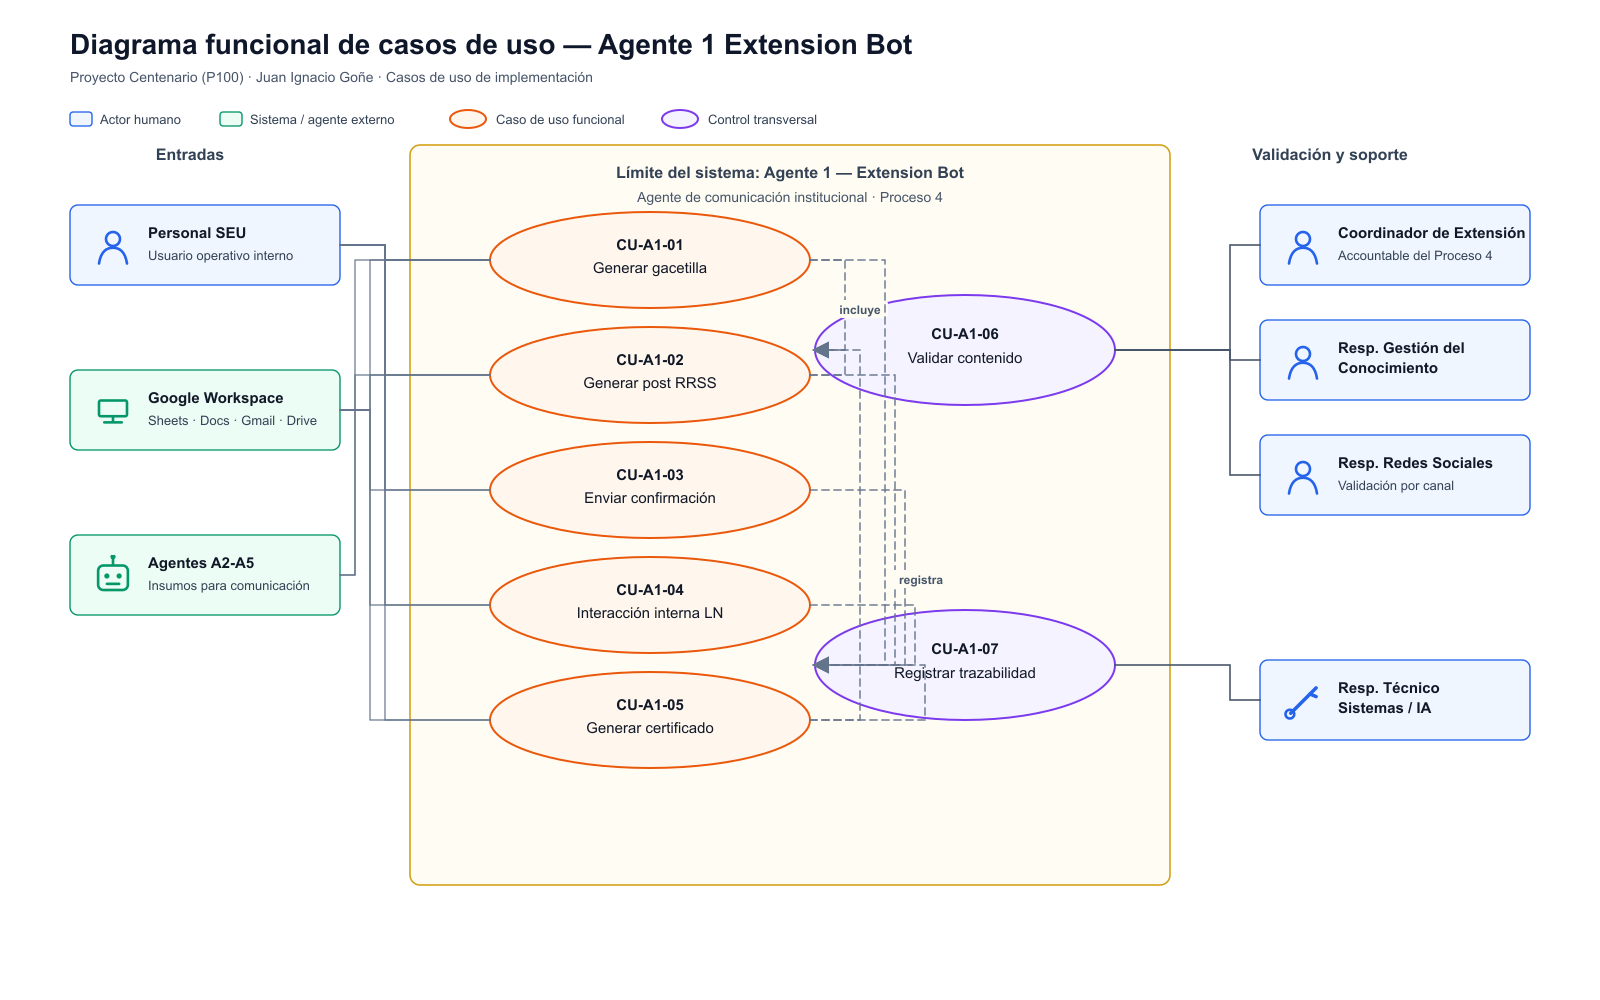
\includegraphics[width=\textwidth]{diagrama-casos-uso-agente-1.png}
  \caption{Diagrama funcional de casos de uso del Agente 1}
  \label{fig:casos-uso-a1}
\end{figure}

\subsection{Lectura del diagrama}

El diagrama se organiza en tres zonas:

\begin{itemize}
  \item \textbf{Entradas}: actores humanos o sistemas que disparan la funcionalidad. Incluyen al Personal SEU, Google Workspace y los agentes A2-A5.
  \item \textbf{Límite del sistema}: contiene los casos de uso ejecutados por el Agente 1. Se distingue entre casos funcionales y controles transversales.
  \item \textbf{Validación y soporte}: actores que aprueban, observan, rechazan o auditan los resultados.
\end{itemize}

Los óvalos funcionales representan valor directo para el usuario: generación de gacetillas, posts, confirmaciones, interacción interna y certificados. Los óvalos transversales no son funcionalidades nuevas del negocio, sino controles obligatorios para que las funcionalidades sean defendibles: \caso{CU-A1-06 Validar contenido} y \caso{CU-A1-07 Registrar trazabilidad}.

\section{Actores}

\begin{longtable}{p{0.26\textwidth}p{0.18\textwidth}p{0.48\textwidth}}
\toprule
\textbf{Actor} & \textbf{Tipo} & \textbf{Rol en el sistema} \\
\midrule
\endhead
Personal SEU & Humano interno & Carga datos, solicita contenidos, revisa salidas operativas y usa al agente en tareas de comunicación institucional. \\
Coordinador de Extensión & Humano interno & Responsable final del Proceso 4. Aprueba pertinencia y utilidad de contenidos antes de difusión masiva. \\
Responsable de Gestión del Conocimiento & Humano interno & Valida coherencia, exactitud, tono institucional y reutilización de contenidos. \\
Responsable de Redes Sociales & Humano interno & Revisa adecuación de posts a canal, longitud, tono y formato. \\
Administración / Secretaría & Humano interno & Valida confirmaciones, registros y certificados vinculados a inscripción o cierre de actividades. \\
Responsable Técnico Sistemas / IA & Humano técnico & Mantiene automatización, permisos, logs, integración y resolución de errores técnicos. \\
Google Workspace & Sistema externo institucional & Provee Sheets, Docs, Drive, Gmail, Forms y Apps Script como infraestructura operativa. \\
Agentes A2-A5 & Sistemas P100 & Aportan insumos: contenido histórico, eventos, respuestas complejas o texto enriquecido. No son orquestados por A1. \\
Destinatarios externos & Público destinatario & Reciben comunicaciones ya validadas. No interactúan directamente con A1 en el alcance vigente. \\
\bottomrule
\end{longtable}

\section{Relaciones entre casos de uso}

\subsection{Relaciones de disparo}

El Personal SEU puede iniciar los cinco casos funcionales principales. En la práctica, esto significa que el agente debe ser operable por usuarios internos sin exigir conocimiento técnico: cargar datos en una planilla, seleccionar una actividad, pedir una pieza de comunicación o solicitar un certificado.

Google Workspace también actúa como disparador porque el flujo del P100 es event-driven: una fila nueva, un formulario, una plantilla o un correo pueden iniciar una ejecución. Esta relación sostiene el bajo costo y la adopción institucional, porque se apoya en herramientas ya conocidas por la Secretaría.

Los agentes A2-A5 se relacionan principalmente con \caso{CU-A1-01} y \caso{CU-A1-02}. Esa relación expresa que A1 puede transformar insumos de otros agentes en comunicación institucional. Por ejemplo, una efeméride proveniente de A2 o un evento detectado por A3 puede convertirse en gacetilla o post. Esta relación no convierte a A1 en orquestador: A1 consume insumos y produce piezas de comunicación.

\subsection{Relaciones de inclusión}

Las relaciones \textit{incluye} indican comportamiento obligatorio reutilizado por varios casos:

\begin{itemize}
  \item \caso{CU-A1-01 Generar gacetilla} incluye \caso{CU-A1-06 Validar contenido}.
  \item \caso{CU-A1-02 Generar post RRSS} incluye \caso{CU-A1-06 Validar contenido}.
  \item \caso{CU-A1-05 Generar certificado} incluye \caso{CU-A1-06 Validar contenido}.
\end{itemize}

La inclusión es necesaria porque estos productos pueden tener impacto reputacional, institucional o administrativo. El agente genera borradores, pero no decide por la Secretaría. La validación humana opera como barrera de calidad frente a errores de datos, tono no adecuado o hallucinations.

\subsection{Relaciones de trazabilidad}

Todos los casos funcionales registran trazabilidad mediante \caso{CU-A1-07}. La relación \textit{registra} significa que cada ejecución debe dejar evidencia mínima: fuente de datos, usuario o trigger, resultado, estado, error si existió y validación cuando corresponda.

Esta relación es transversal porque no alcanza con que el sistema ``funcione''. Para el Proyecto Centenario debe poder demostrarse qué ocurrió, cuándo ocurrió, qué salida produjo y quién la validó. Ese registro alimenta pruebas, auditoría interna y evidencia para evaluación académica.

\subsection{Relaciones de validación y soporte}

\caso{CU-A1-06 Validar contenido} se asocia con Coordinador de Extensión, Responsable de Gestión del Conocimiento y Responsable de Redes Sociales. La distribución depende del tipo de salida:

\begin{itemize}
  \item una gacetilla requiere control de pertinencia institucional y calidad comunicacional;
  \item un post requiere además adecuación al canal de redes sociales;
  \item un certificado requiere validación administrativa antes de emisión;
  \item un mail o confirmación requiere verificación de plantilla, destinatario y registro de envío.
\end{itemize}

\caso{CU-A1-07 Registrar trazabilidad} se asocia al Responsable Técnico de Sistemas / IA porque su cumplimiento depende de logs, permisos, estructuras de datos y mecanismos de auditoría. Sin embargo, la evidencia registrada también debe ser comprensible para los responsables funcionales.

\section{Casos de uso detallados}

\subsection{CU-A1-01: Generar gacetilla institucional}

\begin{tabularx}{\textwidth}{p{0.28\textwidth}Y}
\toprule
\textbf{Campo} & \textbf{Descripción} \\
\midrule
Historia vinculada & HU-010: como Secretaría, quiero generar automáticamente gacetillas para reducir tiempos de redacción. \\
Prioridad & P0. \\
Semestre / TRL & Semestre 1 / TRL 3. \\
Proceso BPM & P4 - Comunicación y Difusión Institucional. \\
Actor primario & Personal de Secretaría de Extensión. \\
Actores secundarios & Coordinador de Extensión, Responsable de Gestión del Conocimiento, Google Sheets, Google Docs y Google Drive. \\
Resultado esperado & Documento Google Docs con borrador de gacetilla institucional, basado en plantilla y datos fuente. \\
\bottomrule
\end{tabularx}

\subsubsection{Descripción extendida}

Este caso de uso automatiza una de las tareas centrales de comunicación institucional: redactar una gacetilla a partir de datos de una actividad, curso, evento u oportunidad de extensión. El valor operativo está en reducir el tiempo inicial de redacción y estandarizar formato, tono y estructura, sin eliminar la revisión humana.

La entrada típica proviene de una planilla Google Sheets. El Agente 1 toma esos datos, genera el texto en registro institucional y produce un documento editable. La gacetilla no queda publicada ni enviada por el solo hecho de ser generada: pasa a estado borrador o pendiente de validación.

\subsubsection{Flujo principal}

\begin{enumerate}
  \item El usuario carga o selecciona una actividad en Google Sheets.
  \item El sistema valida que los campos mínimos estén completos.
  \item Apps Script o el backend envía los datos al Agente 1.
  \item El agente genera un borrador con tono institucional.
  \item El sistema crea un Google Docs aplicando plantilla institucional.
  \item El documento queda pendiente de validación.
  \item El Responsable de Gestión del Conocimiento revisa coherencia y exactitud.
  \item El Coordinador de Extensión aprueba, observa o rechaza.
  \item El sistema registra estado, fecha, usuario validador y vínculo al documento.
\end{enumerate}

\subsubsection{Alternativas y excepciones}

\begin{itemize}
  \item Si faltan datos obligatorios, el sistema marca la solicitud como incompleta.
  \item Si la plantilla no está disponible, no debe usarse para difusión oficial.
  \item Si el texto contiene información dudosa, debe observarse o rechazarse.
  \item Si falla la creación del documento, se registra error técnico y queda pendiente de reintento.
\end{itemize}

\subsubsection{DoD y evidencia}

El caso se considera cerrado cuando existe input desde Sheets, output en Google Docs, plantilla aplicada, texto coherente, ausencia de información inventada, validación humana y log de ejecución. La evidencia esperada incluye documento generado, checklist de validación, fila de control y log.

\subsection{CU-A1-02: Generar post para redes sociales}

\begin{tabularx}{\textwidth}{p{0.28\textwidth}Y}
\toprule
\textbf{Campo} & \textbf{Descripción} \\
\midrule
Historia vinculada & HU-011: como sistema, quiero generar posts para redes para difundir actividades. \\
Prioridad & P0. \\
Semestre / TRL & Semestre 1 / TRL 3. \\
Proceso BPM & P4 - Comunicación y Difusión Institucional. \\
Actor primario & Responsable de Redes Sociales o Personal SEU. \\
Actores secundarios & Responsable de Gestión del Conocimiento, Coordinador de Extensión y Google Workspace. \\
Resultado esperado & Borrador de post adaptado a Instagram y/o LinkedIn. \\
\bottomrule
\end{tabularx}

\subsubsection{Descripción extendida}

Este caso de uso transforma información institucional en piezas breves de difusión digital. Su diferencia principal respecto de la gacetilla es la adaptación al canal: un post para Instagram no tiene la misma longitud, tono ni estructura que una publicación para LinkedIn. Por eso el caso debe admitir canal, objetivo, público destinatario y restricciones de longitud.

El Agente 1 produce propuestas de copy, pero la decisión editorial queda en manos del responsable de comunicación. Cuando el contenido proviene de otros agentes, A1 actúa como normalizador comunicacional: recibe un insumo y lo convierte en lenguaje apto para difusión institucional.

\subsubsection{Flujo principal}

\begin{enumerate}
  \item El usuario selecciona actividad, canal y objetivo comunicacional.
  \item El sistema recupera datos fuente y restricciones del canal.
  \item El Agente 1 genera una versión por canal solicitado.
  \item El borrador se guarda en el repositorio definido.
  \item El Responsable de Redes Sociales valida longitud, tono y formato.
  \item El responsable funcional valida consistencia institucional cuando corresponda.
  \item El sistema registra estado y observaciones.
\end{enumerate}

\subsubsection{Alternativas y excepciones}

\begin{itemize}
  \item Si el canal no está configurado, se solicita selección de un canal definido.
  \item Si la longitud excede el límite, el agente genera versión abreviada.
  \item Si la fuente es insuficiente, el post queda no publicable.
  \item Si el tono no es institucional, el borrador vuelve a edición o regeneración.
\end{itemize}

\subsubsection{DoD y evidencia}

Debe existir formato adaptable a Instagram y LinkedIn, texto limpio y coherente, longitud configurable, adaptación al canal, ausencia de hallucinations, revisión por usuario y log. La evidencia esperada es el post generado, checklist de redes y registro de aprobación u observación.

\subsection{CU-A1-03: Enviar confirmación automática de inscripción}

\begin{tabularx}{\textwidth}{p{0.28\textwidth}Y}
\toprule
\textbf{Campo} & \textbf{Descripción} \\
\midrule
Historia vinculada & HU-012: como Secretaría, quiero enviar confirmaciones automáticas de inscripción para evitar tareas manuales. \\
Prioridad & P1. \\
Semestre / TRL & Semestre 2 / TRL 4. \\
Proceso BPM & P5 - Gestión de Programas, Cursos y Diplomaturas, con soporte comunicacional de P4. \\
Actor primario & Google Workspace mediante trigger de inscripción. \\
Actores secundarios & Personal SEU, destinatario inscripto, Gmail y Google Sheets. \\
Resultado esperado & Email de confirmación enviado y registro de envío actualizado. \\
\bottomrule
\end{tabularx}

\subsubsection{Descripción extendida}

Este caso de uso automatiza una comunicación operativa frecuente: confirmar que una inscripción fue recibida. A diferencia de una gacetilla o post, la confirmación puede ejecutarse automáticamente si parte de una plantilla previamente validada y si los datos de inscripción son correctos.

La automatización no elimina controles: debe evitar duplicaciones, validar correo electrónico, registrar resultado y permitir auditoría. El valor principal está en reducir tareas repetitivas y mejorar la respuesta al inscripto.

\subsubsection{Flujo principal}

\begin{enumerate}
  \item Se registra una nueva inscripción mediante formulario o planilla.
  \item Un trigger detecta la fila pendiente de confirmación.
  \item El sistema valida campos mínimos y verifica que no exista envío previo.
  \item El Agente 1 completa el correo desde plantilla.
  \item Gmail envía el mensaje al destinatario.
  \item La planilla registra fecha, destinatario, estado y error si existió.
  \item La Secretaría puede consultar enviados, fallidos y pendientes.
\end{enumerate}

\subsubsection{Alternativas y excepciones}

\begin{itemize}
  \item Si el email es inválido, no se envía y queda marcado para revisión.
  \item Si la inscripción está duplicada, se evita un segundo envío.
  \item Si falla Gmail o permisos, se registra error y queda pendiente de reintento.
  \item Si la plantilla no está aprobada, el flujo no debe operar en entorno real.
\end{itemize}

\subsubsection{DoD y evidencia}

El caso requiere trigger configurado, email generado automáticamente, registro de envío, manejo de errores, ausencia de duplicaciones y prueba real validada. La evidencia esperada incluye email recibido, fila actualizada y log de ejecución.

\subsection{CU-A1-04: Interacción interna en lenguaje natural}

\begin{tabularx}{\textwidth}{p{0.28\textwidth}Y}
\toprule
\textbf{Campo} & \textbf{Descripción} \\
\midrule
Historia vinculada & HU-013: como usuario interno, quiero interactuar con el agente en lenguaje natural para generar contenido rápidamente. \\
Prioridad & P1. \\
Semestre / TRL & Semestre 2 / TRL 4. \\
Proceso BPM & P4 - Comunicación y Difusión Institucional. \\
Actor primario & Usuario interno de la Secretaría. \\
Actores secundarios & Gmail, interfaz simple o chat interno, Google Sheets. \\
Resultado esperado & Respuesta usable para generación, adaptación o ajuste de contenido institucional. \\
\bottomrule
\end{tabularx}

\subsubsection{Descripción extendida}

Este caso de uso habilita una interacción más flexible que la carga estructurada de planillas. El usuario interno puede pedir un borrador, una reformulación, un resumen o una adaptación de tono. La interacción sigue siendo interna: no es un chatbot público ni una ventanilla de atención masiva.

La relevancia del caso está en reducir fricción para usuarios no técnicos. Sin embargo, también es uno de los casos que más requiere control de alcance, porque una interfaz en lenguaje natural puede recibir pedidos fuera del rol del Agente 1.

\subsubsection{Flujo principal}

\begin{enumerate}
  \item El usuario interno envía una solicitud por el canal definido.
  \item El sistema verifica usuario y alcance de la solicitud.
  \item El Agente 1 interpreta el pedido y detecta datos faltantes.
  \item Si la información es suficiente, genera una respuesta usable.
  \item El sistema registra interacción, entrada y salida.
  \item El usuario revisa la respuesta y decide si la incorpora a un flujo formal.
\end{enumerate}

\subsubsection{Alternativas y excepciones}

\begin{itemize}
  \item Si el pedido corresponde a atención pública, se deriva al alcance de A4.
  \item Si solicita analítica, KPIs o scraping, se rechaza por fuera de alcance o se deriva a A5.
  \item Si faltan datos verificables, el agente solicita información adicional.
  \item Si el usuario no tiene permisos, no se procesa la solicitud.
\end{itemize}

\subsubsection{DoD y evidencia}

El caso exige interfaz simple, respuesta usable, registro de interacción, control básico de alcance y ausencia de información inventada. La evidencia esperada es una captura o registro de prueba guiada, junto con log de la interacción.

\subsection{CU-A1-05: Generar certificado automático con validación humana}

\begin{tabularx}{\textwidth}{p{0.28\textwidth}Y}
\toprule
\textbf{Campo} & \textbf{Descripción} \\
\midrule
Historia vinculada & HU-014: como Secretaría, quiero generar certificados automáticos para agilizar cierres de actividades. \\
Prioridad & P2. \\
Semestre / TRL & Semestre 2 / TRL 4. \\
Proceso BPM & P5 - Gestión de Programas, Cursos y Diplomaturas, con soporte documental de P4. \\
Actor primario & Personal SEU o Administración. \\
Actores secundarios & Coordinador de Extensión, Google Sheets, Google Drive y generador PDF. \\
Resultado esperado & Certificado PDF generado desde plantilla, pendiente o aprobado para emisión. \\
\bottomrule
\end{tabularx}

\subsubsection{Descripción extendida}

Este caso genera certificados a partir de datos validados de una actividad. Es más sensible que una pieza de difusión porque puede tener implicancias administrativas y académicas. Por eso la validación humana previa es obligatoria y no puede omitirse.

El Agente 1 automatiza la preparación del documento, pero no decide quién debe recibirlo ni certifica por sí mismo que una persona cumplió condiciones de asistencia o aprobación. Esa validación corresponde al circuito institucional definido por la Secretaría.

\subsubsection{Flujo principal}

\begin{enumerate}
  \item El usuario selecciona actividad y destinatarios.
  \item El sistema valida datos mínimos: nombre, actividad, condición, fecha y plantilla.
  \item El Agente 1 completa la plantilla de certificado.
  \item El sistema genera un PDF preliminar por destinatario o por lote.
  \item Administración o responsable definido revisa exactitud.
  \item El validador aprueba, observa o rechaza.
  \item El sistema registra estado de cada certificado.
  \item Solo los certificados aprobados quedan disponibles para emisión o envío.
\end{enumerate}

\subsubsection{Alternativas y excepciones}

\begin{itemize}
  \item Si faltan datos, el certificado queda bloqueado.
  \item Si la plantilla no está aprobada, no hay generación oficial.
  \item Si falla el PDF, se registra error técnico.
  \item Si el validador rechaza, no se emite.
\end{itemize}

\subsubsection{DoD y evidencia}

Debe existir plantilla base, generación PDF, validación humana previa, registro de estado por certificado y log. La evidencia incluye PDF generado, registro de aprobación u observación y planilla de control.

\subsection{CU-A1-06: Validar contenido generado}

\caso{CU-A1-06} es transversal. No representa una funcionalidad opcional, sino un control obligatorio para proteger calidad institucional y evitar automatización indebida. Se aplica especialmente a gacetillas, posts, certificados y comunicaciones oficiales.

\subsubsection{Flujo principal}

\begin{enumerate}
  \item El sistema presenta el borrador o certificado al responsable.
  \item El responsable revisa datos, tono, formato, canal y consistencia institucional.
  \item El responsable aprueba, observa o rechaza.
  \item El sistema registra decisión, fecha, usuario y observaciones.
  \item El contenido aprobado avanza al paso operativo siguiente.
\end{enumerate}

\subsubsection{Criterio de control}

La validación humana debe impedir que el agente publique, envíe comunicaciones críticas o emita documentos oficiales sin intervención responsable. Esto preserva el principio de asistencia: la IA amplía capacidad operativa, pero no sustituye el juicio institucional.

\subsection{CU-A1-07: Registrar trazabilidad}

\caso{CU-A1-07} es el segundo control transversal. Su función es generar evidencia verificable de ejecución, resultados y validaciones. Sin este caso, las historias podrían parecer funcionales en una demostración, pero no serían defendibles frente a auditoría o evaluación académica.

\subsubsection{Flujo principal}

\begin{enumerate}
  \item El sistema inicia una ejecución.
  \item Registra identificador, fecha, usuario o trigger y fuente de datos.
  \item Registra resultado técnico: exitoso, observado, rechazado, fallido o pendiente.
  \item Si existe validación humana, registra validador, decisión y observación.
  \item El Responsable Técnico puede auditar logs y reportar errores.
\end{enumerate}

\subsubsection{Criterio de control}

La evidencia debe permitir reconstruir qué se generó, desde qué fuente, con qué estado y bajo qué validación. Los logs no deben exponer credenciales ni datos sensibles innecesarios.

\section{Matriz de trazabilidad}

\begingroup
\small
\setlength{\tabcolsep}{2pt}
\begin{longtable}{@{}p{0.16\textwidth}p{0.12\textwidth}p{0.15\textwidth}p{0.12\textwidth}p{0.25\textwidth}p{0.08\textwidth}@{}}
\toprule
\textbf{Elemento} & \textbf{Proceso} & \textbf{Historia} & \textbf{Caso} & \textbf{Evidencia esperada} & \textbf{Estado} \\
\midrule
\endhead
Gacetilla institucional & P4 & HU-010 & CU-A1-01 & Documento generado, checklist, log & Borrador \\
Post RRSS & P4 & HU-011 & CU-A1-02 & Post generado, checklist RRSS, log & Borrador \\
Confirmación de inscripción & P5 + P4 soporte & HU-012 & CU-A1-03 & Email recibido, fila Sheets, log & Borrador \\
Interacción interna LN & P4 & HU-013 & CU-A1-04 & Captura de interacción, salida generada, log & Borrador \\
Certificado automático & P5 + P4 soporte & HU-014 & CU-A1-05 & PDF generado, aprobación, log & Borrador \\
Validación humana & P4 / P5 & Control transversal & CU-A1-06 & Estado aprobado, observado o rechazado & Borrador \\
Trazabilidad & Transversal CONEAU & DoD global & CU-A1-07 & Log estructurado y vínculo a salidas & Borrador \\
\bottomrule
\end{longtable}
\endgroup

\section{Reglas de negocio derivadas}

\begin{enumerate}
  \item Todo contenido institucional generado por el Agente 1 queda como borrador hasta validación humana.
  \item El agente no debe inventar datos faltantes; debe solicitar corrección o marcar el caso como incompleto.
  \item Los destinatarios externos no son usuarios directos del Agente 1 durante el alcance vigente.
  \item La Secretaría conserva responsabilidad institucional sobre aprobación, publicación, envío oficial y emisión de certificados.
  \item Toda automatización debe dejar evidencia verificable.
  \item Analítica, scraping, dashboards y atención pública masiva quedan fuera del Agente 1.
  \item Las integraciones con A2-A5 son relaciones de insumo, no de orquestación funcional por parte de A1.
\end{enumerate}

\section{Datos mínimos por caso}

\begin{longtable}{p{0.18\textwidth}p{0.46\textwidth}p{0.28\textwidth}}
\toprule
\textbf{Caso} & \textbf{Datos mínimos de entrada} & \textbf{Salida esperada} \\
\midrule
\endhead
CU-A1-01 & Nombre de actividad, descripción, fecha, destinatarios, responsable, contacto y fuente institucional. & Google Docs de gacetilla. \\
CU-A1-02 & Actividad o contenido, canal, objetivo, fecha, público destinatario y restricciones de longitud. & Borrador de post por canal. \\
CU-A1-03 & Nombre del inscripto, email, actividad, fecha/hora y estado de inscripción. & Email de confirmación y registro. \\
CU-A1-04 & Solicitud del usuario, contexto, canal deseado y datos fuente disponibles. & Respuesta interna usable o pedido de datos faltantes. \\
CU-A1-05 & Nombre del destinatario, actividad, condición, fecha, autoridad o firmante si aplica y plantilla. & PDF de certificado pendiente o aprobado. \\
\bottomrule
\end{longtable}

\section{Pendientes de confirmación}

Antes de considerar esta especificación cerrada para implementación, deben confirmarse:

\begin{itemize}
  \item campos definitivos de Google Sheets para actividades, inscripciones y certificados;
  \item plantillas institucionales finales para gacetillas, posts, mails y certificados;
  \item responsable nominal de cada validación operativa;
  \item instrumento formal de checklist y escala de validación;
  \item canal exacto de interacción interna para HU-013;
  \item ubicación final y formato estructurado de logs;
  \item fechas oficiales de revisión y validación académica.
\end{itemize}

\section{Conclusión}

Los casos de uso definidos muestran que el Agente 1 concentra valor en la generación asistida de comunicaciones institucionales y documentos operativos, pero su diseño depende de dos controles transversales: validación humana y trazabilidad. La primera evita que la IA sustituya decisiones institucionales; la segunda permite demostrar uso, calidad y control ante evaluación académica.

La relación entre casos funcionales y controles transversales es, por lo tanto, central para la defensa del proyecto. El Agente 1 no debe medirse únicamente por la cantidad de textos que genera, sino por su capacidad de integrarse al Proceso 4, respetar roles RACI, producir evidencia y operar dentro de los límites definidos para el Proyecto Centenario.

\end{document}
